\section{Analysis}

The average age of pitchers was 30 years old and average FIP scores were similar for index year and year prior as seen in Table \ref{tbl:desc-stats}. None of these variables showed a significant difference in logistic regression.

\begin{table}[h]
\centering
\caption{Average age and FIP score for pitchers}
\label{tbl:desc-stats}
\begin{tabular}{clll}
     & Means & SD (+/-)  \\
Age  & 30    & 3.8  \\
FIPx & 4.37  & 1.9  \\
FIPy & 4.23  & 1.68
\end{tabular}
\end{table}

Table \ref{tbl:conf-matrix} shows a confusion matrix on the prediction of our random forest. An accuracy of 52.38\% was reported but this was mostly due to the model failing to predict anything as a TJS. The 95\% confidence intervals reported for this accuracy was 29.78\% to 74.29\%. This large spread also shows the model was essentially unable to properly classify the data.

\begin{table}[h]
\centering
\caption{Confusion matrix for random forest conducted on our dataset}
\label{tbl:conf-matrix}
\begin{tabular}{lll}
           & \multicolumn{2}{l}{Reference} \\
Prediction & 0             & 1             \\
0          & 8             & 1             \\
1          & 9             & 3
\end{tabular}
\end{table}

Given that our data set was unable to provide any valid results we decided to run a random forest analysis on a small dataset previously collected and provided by RockFence LLC. The exact details of how the data were collected were not provided by the company, however verbal confirmation on previous results were provided. As per our conversation with their representative they advised that logistic regression also showed no significant results worth reporting but a random tree show some factors of interest albeit very minimal. As such we attempted to run a random forest on the same data set so we had some valuable data to present in this report.

\begin{table}[h]
\centering
\caption{Confusion matrix for random forest conducted on RockFence LLC provided dataset}
\label{tbl:rockfence}
\begin{tabular}{lll}
           & \multicolumn{2}{l}{Reference} \\
Prediction & 0              & 1            \\
0          & 124            & 5            \\
1          & 46             & 16
\end{tabular}
\end{table}

As seen in table \ref{tbl:rockfence} their model was also a poor predictor of TJS pitchers. This models accuracy was reported as 73.30\% with 95\% confidence intervals between 66.43\% and 79.43\%. The high number of correct classifications could be a result of more non TJS pitchers being in the dataset and thus classifying the majority of the pitchers as non TJS will appear to have a high accuracy.

\begin{figure}[h]
    \centering
        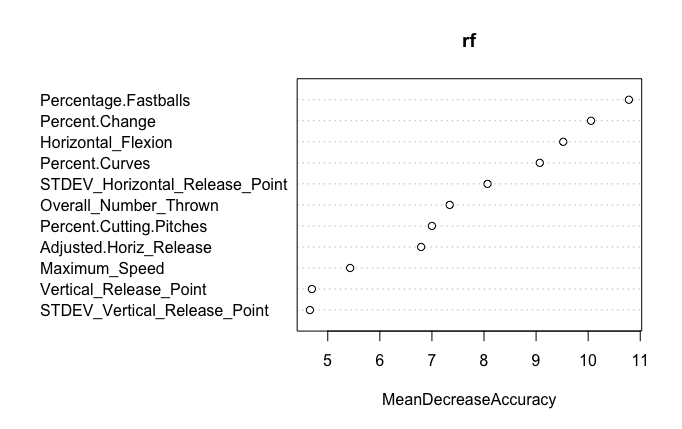
\includegraphics[width=0.5\textwidth]{meanDecreaseAccuracy}
    \caption{Mean decrease accuracy showing how variables affect the accuracy of the model}
    \label{fig:mda}
\end{figure}

The general idea of mean decrease accuracy as shown in Figure \ref{fig:mda} is to permute the values of each feature and measure how much the permutation decreases the accuracy of the model. Therefore, for unimportant variables, the permutation should have little to no effect on model accuracy, while permuting important variables should significantly decrease it.

\begin{figure}[h]
    \centering
        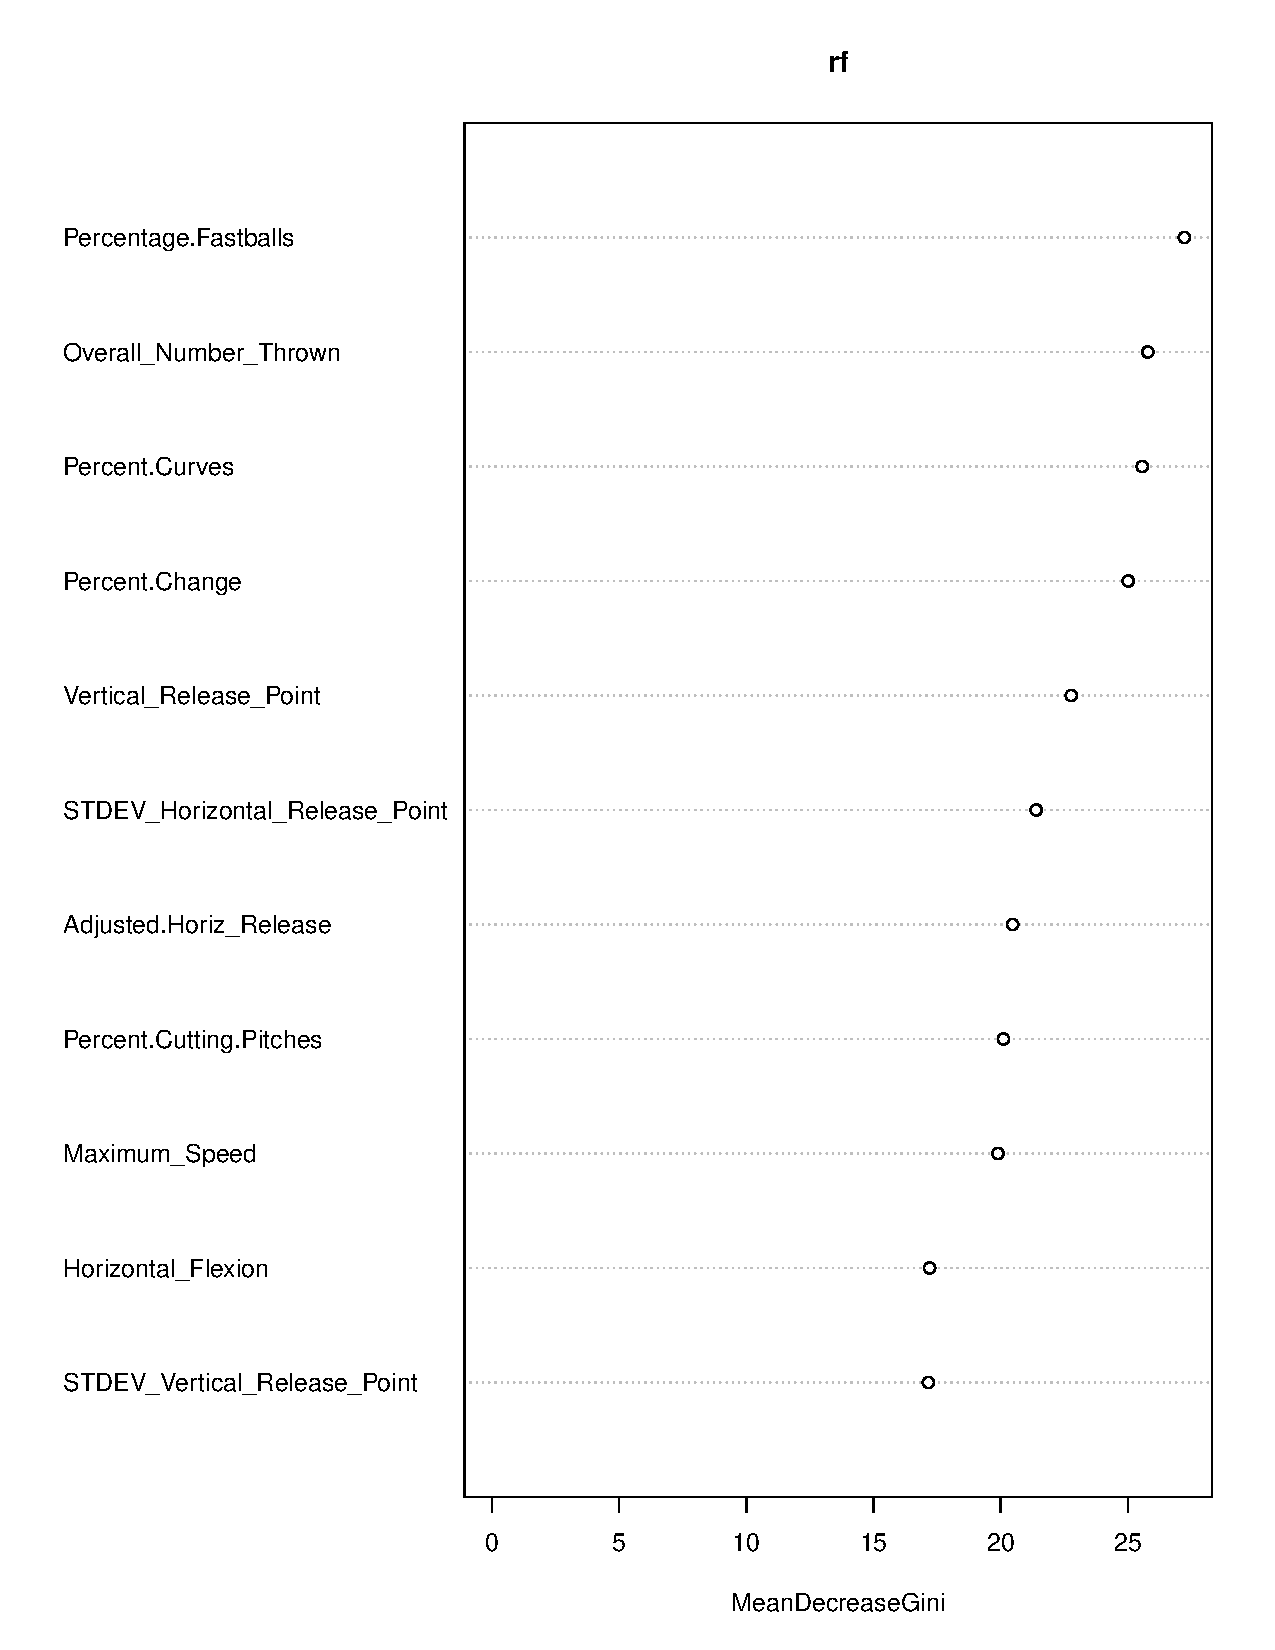
\includegraphics[width=0.5\textwidth]{meanDecreaseGINI}
    \caption{Mean decrease impurity showing how often elements can affect the model if chosen randomly}
    \label{fig:mdg}
\end{figure}

Figure \ref{fig:mdg} shows the mean decrease impurity which uses the R function varImpPlot to measure the mean decrease GINI impurity.Gini impurity is a measure of how often a randomly chosen element from the set would be incorrectly labeled if it were randomly labeled according to the distribution of labels in the subset.

The RockFence LLC supplied data corresponds with other previously reported cases that the number of fastballs thrown is an important factor in predicting TJS surgery.